% ==============================================================================
% Chapter 2: Karnaugh Map - Spot-the-difference
% ==============================================================================
\section{Karnaugh Map (spot-the-difference)}

\begin{hack}[K-Map is just a spot-the-difference game]
\textbf{Three steps:}
\begin{enumerate}
\item \textbf{Fill the map:} set cells to 1 according to minterms
\item \textbf{Group the 1s:} circle them (bigger is better)
\item \textbf{Write terms:} for each group, write the variables that do not change
\end{enumerate}
\end{hack}

\subsection{4-variable K-Map template (copy it)}

\begin{center}
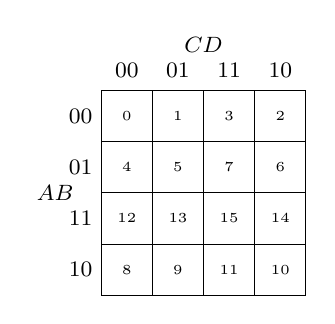
\begin{tikzpicture}[scale=0.65]
\draw (0,0) grid (4,4);
% Column labels CD
\node at (0.5, 4.4) {\footnotesize 00};
\node at (1.5, 4.4) {\footnotesize 01};
\node at (2.5, 4.4) {\footnotesize 11};
\node at (3.5, 4.4) {\footnotesize 10};
\node at (2, 4.9) {\footnotesize $CD$};
% Row labels AB
\node at (-0.4, 3.5) {\footnotesize 00};
\node at (-0.4, 2.5) {\footnotesize 01};
\node at (-0.4, 1.5) {\footnotesize 11};
\node at (-0.4, 0.5) {\footnotesize 10};
\node at (-0.9, 2) {\footnotesize $AB$};
% Indices
\node at (0.5,3.5) {\tiny 0};
\node at (1.5,3.5) {\tiny 1};
\node at (2.5,3.5) {\tiny 3};
\node at (3.5,3.5) {\tiny 2};
\node at (0.5,2.5) {\tiny 4};
\node at (1.5,2.5) {\tiny 5};
\node at (2.5,2.5) {\tiny 7};
\node at (3.5,2.5) {\tiny 6};
\node at (0.5,1.5) {\tiny 12};
\node at (1.5,1.5) {\tiny 13};
\node at (2.5,1.5) {\tiny 15};
\node at (3.5,1.5) {\tiny 14};
\node at (0.5,0.5) {\tiny 8};
\node at (1.5,0.5) {\tiny 9};
\node at (2.5,0.5) {\tiny 11};
\node at (3.5,0.5) {\tiny 10};
\end{tikzpicture}
\end{center}

\textbf{Gray code order: 00, 01, 11, 10} (memorize)

\subsection{How to fill the map}

\begin{hack}[Where does each variable go?]
\textbf{Regions for ABCD in a 4-variable map:}
\begin{itemize}
\item $A=1$: bottom two rows (row 11, 10)
\item $B=1$: middle two rows (row 01, 11)
\item $C=1$: middle two columns (col 01, 11)
\item $D=1$: right two columns (col 11, 10)
\end{itemize}

\textbf{Negation:} $\bar{A}$ means the $A=0$ region.
\end{hack}

\subsection{Grouping with no-brain patterns}

\begin{hack}[Four must-know grouping patterns]
\textbf{1. Four corners} = $\bar{B}\bar{D}$
\begin{center}
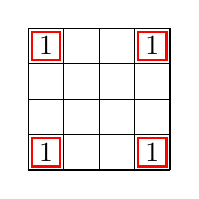
\begin{tikzpicture}[scale=0.45]
\draw (0,0) grid (4,4);
\node at (0.5,3.5) {1}; \node at (3.5,3.5) {1};
\node at (0.5,0.5) {1}; \node at (3.5,0.5) {1};
\draw[red,thick] (0.1,3.1) rectangle (0.9,3.9);
\draw[red,thick] (3.1,3.1) rectangle (3.9,3.9);
\draw[red,thick] (0.1,0.1) rectangle (0.9,0.9);
\draw[red,thick] (3.1,0.1) rectangle (3.9,0.9);
\end{tikzpicture}
\end{center}

\textbf{2. Whole row} = only AB changes
\begin{center}
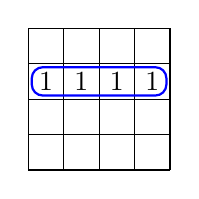
\begin{tikzpicture}[scale=0.45]
\draw (0,0) grid (4,4);
\node at (0.5,2.5) {1}; \node at (1.5,2.5) {1};
\node at (2.5,2.5) {1}; \node at (3.5,2.5) {1};
\draw[blue,thick,rounded corners] (0.1,2.1) rectangle (3.9,2.9);
\end{tikzpicture}
\end{center}

\textbf{3. 2x2 block (4 cells)} = eliminates two variables

\textbf{4. Wrap-around (top/bottom or left/right)} = groups may cross edges
\end{hack}

\subsection{Grouping rules}

\begin{pitfall}[Three iron rules]
\begin{enumerate}
\item Group size must be a \textbf{power of two}: 1, 2, 4, 8, 16
\item \textbf{Bigger is better} (eliminate more variables)
\item Every 1 must be \textbf{covered at least once}
\end{enumerate}
\end{pitfall}

\subsection{Write the expression from a group}

\begin{hack}[Write what does not change inside the group]
\textbf{Look at variable values within the group:}
\begin{itemize}
\item always 1 $\to$ write the variable
\item always 0 $\to$ write the negated variable
\item sometimes 0 sometimes 1 $\to$ omit it (it cancels)
\end{itemize}

\textbf{Example:} group at AB=01, CD=any
\begin{itemize}
\item A is always 0 $\to$ write $\bar{A}$
\item B is always 1 $\to$ write $B$
\item C and D vary $\to$ omit
\item \textbf{Result: $\bar{A}B$}
\end{itemize}
\end{hack}

\subsection{The XOR secret}

\begin{hack}[Checkerboard pattern = XOR]
If the 1s and 0s alternate like a chessboard:

\begin{center}
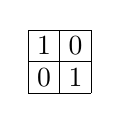
\begin{tikzpicture}[scale=0.4]
\draw (0,0) grid (2,2);
\node at (0.5,1.5) {1}; \node at (1.5,1.5) {0};
\node at (0.5,0.5) {0}; \node at (1.5,0.5) {1};
\end{tikzpicture}
\end{center}

\textbf{Write directly:} $A \oplus B$ (XOR)

This case \textbf{cannot be simplified further}; don't waste time trying to group it.
\end{hack}

\subsection{Don't-care}

\begin{keybox}[X can be treated as 1 or 0]
\begin{itemize}
\item If it makes a group bigger $\to$ treat as 1
\item Otherwise $\to$ treat as 0 and ignore
\end{itemize}
Goal: make groups as large as possible.
\end{keybox}
